\documentclass{sig-alternate}

\begin{document}

\title{Chemoinformatics: The Computer Science of Chemistry}
\numberofauthors{3}
\author{
\alignauthor
Ben Trovato\titlenote{Dr.~Trovato insisted his name be first.}\\
       \affaddr{Institute for Clarity in Documentation}\\
       \affaddr{1932 Wallamaloo Lane}\\
       \affaddr{Wallamaloo, New Zealand}\\
       \email{trovato@corporation.com}
% 2nd. author
\alignauthor
G.K.M. Tobin\titlenote{The secretary disavows
any knowledge of this author's actions.}\\
       \affaddr{Institute for Clarity in Documentation}\\
       \affaddr{P.O. Box 1212}\\
       \affaddr{Dublin, Ohio 43017-6221}\\
       \email{webmaster@marysville-ohio.com}
% 3rd author
\alignauthor
Rajarshi Guha\\
\affaddr{NIH Center for Translational Therapeutics}\\
\affaddr{9800 Medical Center Drive}\\
\affaddr{Rockvile, MD 20850}\\
\email{guhar@mail.nih.gov}
}

\additionalauthors{Additional authors: John Smith (The Th{\o}rv{\"a}ld Group,
email: {\texttt{jsmith@affiliation.org}}) and Julius P.~Kumquat
(The Kumquat Consortium, email: {\texttt{jpkumquat@consortium.net}}).}
\date{30 July 1999}

\maketitle
\begin{abstract}
  One of the most prominent success stories in all of science over the last decade has
  been the advance of bioinformatics: interdisciplinary collaboration between
  computer scientists and molecular biologists led to the sequencing the human genome
  (among many other accomplishments), because researchers connected biological
  technologies to the theory of string algorithms. However, despite this great
  success, few computer scientists are familiar with a related (and older!)
  discipline -- chemoinformatics, the use of computers to discover new molecules with
  desired behavior, such as new pharmaceuticals or industrial solvents. Until
  recently, the data and techniques of chemoinformatics have been closely guarded
  secrets of companies whose financial success depended on being the first to produce
  the new "miracle molecule". Only within the last decade -- and largely because of
  chemists volunteering their time for an Open Science "movement" -- do researchers
  now have access to freely available software packages and databases of tens of
  millions of chemicals. As a result, chemists now confront hundreds of unsolved
  algorithmic problems that could not have been tackled a decade ago, but whose
  solutions are critical to research ranging from determining the behavior of small
  molecules in biological pathways, to finding a cure for malaria.
\end{abstract}

\category{H.4}{Information Systems Applications}{Miscellaneous}
\terms{Theory}
\keywords{cheminformatics, graphs, chemistry}

\section{Is Cheminformatics the New Bioinformatics?}

Novel technologies in the life sciences churn out information at an ever
increasing rate – public data stores such as at the European Bioinformatics
Institute (EBI) contain on the order of 10 Petabytes of biological information,
a long way from the few kilobytes of the first sequenced genome in 1977.
However, while biological information has been available publicly for decades,
the same has not been true for chemical information until very recently. Only
2004 saw a large public compound repository, PubChem, entering the public
domain, followed more recently by other databases as discussed later in this
article. In the same vein, open source software and the publication of
algorithms have only recently become a main focus of the field \cite{faulon2010}.

So why should we actually care about chemical information being made public --
and how does this relate to the field of computer science?

Both of these questions have relatively straightforward answers. We should care
about chemical information being made public since the drugs we take are the
result of intensive and costly research, and the more information is shared (a
process sometimes very hard to achieve in pharmaceutical companies) the more
easy it should be to develop novel treatments drugs. How chemical information
relates to computer science becomes clear when realizing the amount of data
available currently -- 74 million different molecules with annotations are
currently stored in public databases such as PubChem with a large amount of
annotations, and the design of data structures for chemicals, as well as
subsequent data mining of this information, are areas where expertise in
computer science is dearly needed. (For a recent, detailed introduction to the
field written for computer scientists see \cite{brown2009}). Cheminformatics
comprises different areas, which broadly speaking can be divided into three
fields: capturing data (using lab notebooks or potentially using formats such as
the Chemical Markup Language for publications); storing data (designing database
schemas, devising ontologies) and mining data (such as for bioactivity
prediction, which might involve algorithms based on graphs). However, what is a
major difference to the bioinformatics field is the type of information being
analyzed: While bioinformatics often deals with sequences, the domain of
cheminformatics is chemical structures. In case of the former, information can
very frequently be represented as one-dimensional strings, which are relatively
easy to handle computationally. On the other hand, chemical structures may
possess rings, branches as well as multiple valid representations of even the
same structure, potentially giving rise to ambiguities. Hence, chemical
structure is often thought of as being more difficult to standardize than
information from other domains. As an illustration, different representations of
the same chemical structure are shown in Figure 1. The top left hand corner
shows a structure a chemist would draw it -- every 'corner' representing a carbon
atom (which can also be represented as a C), every O denoting oxygen, every N
nitrogen, every H hydrogen and so on. This is the standard format chemists use
when exchanging information with their peers. However, this is not directly
amenable to data mining -- different atoms might be collapsed into one node,
sets of atoms might have the same relevant properties assigned. Hence, the top
right hand corner of Figure 1 shows an annotated graph representation, taking
into account that atoms, though being of different elemental atom type, can have
similar properties -- e.g. both oxygen and nitrogen carry an 'On' label in this
graph.

% \begin{figure}
% \centering
% \psfig{file=placeholder.ps}
% \caption{The many different facets of representing chemical structures. Shown
% are a chemist’s usually representation of a molecule (top left) and a
% graph-based representation amenable to data mining (top right). These
% representations are supplemented by a 3D representation of the same molecule
% (bottom left) that is closer to reality and a representation using surface
% properties (bottom right), which is often more relevant for the properties the
% molecule exhibits in an experimental setup (such as when measuring its
% solubility, or bioactivity).}
% \end{figure}

On this graph, and employing large databases of thousands of molecules, graph
mining algorithms can be applied to discover patterns in large-scale datasets
and a large number of successful applications of this concept have been
published \cite{wegner2006,horst2009}. Still, this second representation is far
from being the end of the story. Molecules are 3D entities as represented in the
bottom left hand corner of the figure, and the precise 3D shape is relevant in
many situations (while not in others), but this is information that is lost when
only considering the graph of a molecule. To even extend this concept, in many
cases actually the surface properties of theq molecule are what appears to be
relevant in e.g. biological systems, as shown in the bottom right hand corner.
Hence, while graph mining on chemicals is certainly a promising avenue to
explore, one needs to keep in mind that not all molecular properties are encoded
in the graph (such as rotational states, or different charge states etc.) and
thus often other 'descriptors' need to be used to capture the essentials of a
chemical system \cite{bender2004}.

From the above it becomes clear that the nature of chemical problems is often a
complex mixture of combinatorial and continuous problems. If we oversimplify the
nature of chemical structures and their properties we can not describe the world
around us in sufficient details. On the other hand, if we try encoding all
details the complexity to collect, store, and mine data increases dramatically
(e.g. all possible 3D structures and their properties, all metabolites of a
structure in humans in different tissues). For the field of cheminformatics to
flourish, we need closer collaboration between chemists (or, more generally,
life scientists) and computer scientists – where the former needs to be able to
pose the problem in a way relevant for practical applications; and where the
latter is able to devise ways of capturing, storing, and analyzing chemical data
by bridging the gap between risk in generalizable encodings and complexity
(space and time). The goal is supporting a better chemical decision making by
reducing the risks by 1. storing and integrating data in maintainable ways, 2.
providing enough open standards and tools to allow software engineering concepts
to help bridging silos, and 3. mining the many chemical property spaces in a
time and space efficient way. Many aspects pertaining to those areas will be
discussed in the following sections.

\section{Bridging Cheminformatics \& Computer Science}
\label{sec:bridg-chem-}

\subsection{Databases \& Ontologies}
\label{sec:datab--ontol}

Most cheminformatics applications rely on large databases of chemical structures
and their properties. Organising and maintaining such databases, searching based
on features of chemical structures, and clustering similar structures together,
are essential utilities to enable many scientific applications. Yet, each one of
those challenges poses its unique computer science complexities.

There is a considerable progress in open chemical and bioactivity databases like
ChEMBL and NCBI-PubChem, which are both freely available. Still, the integration
of chemical databases with each other remains a challenge, not only due to the
normalization problems in the chemical and bioactivity landscape, but also due
to the sheer data volume of them. As mentioned earlier, we have to be able to
search in complex data, for example multi-labelled molecular graphs, where
labels can be different tautomeric states, different protonation states, or many
variations of implicit chemical expert knowledge we need to capture in a
risk-bounded machine encoded way.

Chemical graphs can differ based on the manner in which the structures are
drawn. Checking whether two graphs represent the same chemical is an expensive
operation (the next section will discuss this in-depth), thus, a representation
of the structure that is unique and invariant with respect to how the structure
is drawn is needed for identification. An early effort in this direction was the
Simplified Molecular Input Line Specification (SMILES). However, several
different implementations became available. After years of research and various
commercial products, is there today not a single public standard for a
line-notation of molecular labelled graphs, which is available to a broad
audience (academic and commercial). The very same problem does also exist for
bioassay ontologies and the lack of options to normalize the property spaces of
chemical compounds, e.g. biological assays or clinical data outcome
(biobanking).
   
With each database using their own algorithm for molecular encoding, little
facilitated the automated exchange of data between different databases. As more
and more data became available online, structure-based identification became a
pressing need, and the IUPAC International Chemical Identifier (InChI) code was
developed. The InChI is a non-proprietary, structured textual identifier for
chemical entities [1]. InChI identifiers are not intended to be read and
understood by humans, but are useful for computational matching of chemical
entities. For rapid database lookups, the InChIKey is a hashed key for the
InChI, which has an invariant length of 14 characters. Figure 1 illustrates the
SMILES, InChI and InChIKey for lipoic acid.

Figure 1: The standard chemical graph illustration together with the SMILES,
InChI and InChIKey codes for lipoic acid. Note that the SMILES is much more
human-readable than the others.

The InChI is now widely used for matching identical chemical structures, but it
is still limited in a few scenarios. For example, it cannot differentiatebetween
certain types of stereoisomers: Figure 2 illustrates two stereoisomers for which
the generated InChI is the same.

Figure 2: The generated InChI is the same for the stereoisomers cisplatin and
transplatin.

InChI or other identity-mapping algorithms allow for exact searching (within the
limitations of the algorithms), but two other requirements for scientific
discovery based on chemical databases are substructure searching and similarity
searching. In substructure searching, the database is searched for a specified
wholly contained part of the structures in the database; in similarity
searching, the database is searched for structures similar to a provided search
structure. Chemical search packages are often implemented and optimised for a
given database technology, for example, the OrChem package is an open source
chemical search package for the Oracle database \cite{rijnbeek2009}.

Graph substructure matching is a variant of graph isomorphism detection,which is
well known to be computationally intractable [3]. To execute a graph isomorphism
search across a full chemical database of thousands or even millions of
structures is completely infeasible. For that reason, complex heuristics must be
used to drastically filter the candidate search space. Structure-based
fingerprints are commonly used for this purpose. Fingerprints encode
characteristic features of a given chemical structure in a boolean array, or
bitmap. The fingerprint is created by an algorithm which generates bitmap
patterns for each atom in the structure; then each atom and its nearest
neighbours, including the bonds between them; then each group of atoms connected
by paths of increasing lengths up to the maximum implemented for the algorithm
(commonly around eight). The bitmap patterns are added together into the final
fingerprint. If all bits in a query fingerprint are also present in the target
fingerprint of a stored database structure, only then is the structure subjected
to the computationally expensive subgraph matching algorithm. Bit operations are
very fast and independent of the number of atoms in a structure due to the fixed
length of the fingerprint.

Fingerprints also facilitate the rapid calculation of quantitative
structure-based similarity measures. An example measure of similarity is the
Tanimoto coefficient, calculated as the ratio $T(a,b) = \frac{c}{(a+b−c)}$,
where c is the count of bits on in the same position in both the two
fingerprints, a is the count of bits on in the first structure, and b is the
count of bits on in the second structure. The Tanimoto coefficient varies in the
range 0.0 -- 1.0, with a score of 1.0 indicating that the two structures are very
similar (i.e. their fingerprints are the same). Structure-based similarity is of
limited use in grouping of chemicals based on non-structural features, such as
shared bioactivity profiles. For this purpose, a large-scale and flexible
classification structure is needed for chemicals and their linked biological
information. One such answer to this need is provided in the form of ontologies.
An ontology is a formal specification of entities and their relationships in a
domain of interest. It is structured around an underlying logical representation
such as Description Logic [baaderdl2007]. The logic-based representation allows
automated reasoning to derive new knowledge (inferences) from the knowledge
encoded, making the representation both compact and immensely powerful.
Ontologies are already in widespread use across the biomedical domain. A
similarity measure based on the information encoded in ontologies is termed
‘semantic similarity, and such measures have already been applied to enhance
chemical classification in several problem areas [couto2010]. Many open
questionsstill remain as to the best way to combine the information encoded in
chemical structures with chemical ontologies [hastingsowled2010].

\subsection{Structure Enumeration}
\label{sec:struct-enum}

Enumerating molecules is a combinatorial problem that has fascinated chemists,
computer scientists and mathematicians alike for more than a century. It is one
important risk-reduction element in still being able to encode closely-related
molecules and for keeping the space complexity of databases under (algorithmic)
control. Indeed, while trying to solve the problem of counting the isomers of
paraffin structures or counting substituted aromatic compounds, fundamental
principles in graph theory and combinatorics were developed by Cayley, Polya and
others. Even terms that are widely-used nowadays like graph and tree were
originally coined in a chemistry context (Chapters 1 and 8 in [1]). More than
four decades ago, Joshua Lederberg, Carl Djerassi, Edward Feigenbaum and others
from Stanford University started developing codes to explicitly enumerate
molecules. Their project named DENDRAL was funded by NASA with the goal of
developing an automated system to elucidate compounds from spectral data. While
studying this challenging problem, important concepts in computer science were
developed. DENDRAL is generally quoted in artificial intelligence textbooks as a
pioneer project that produced the first expert system.
 
Enumerating molecules is not only an interesting academic exercise but has
practical utility as well. The foremost application of enumeration is structure
elucidation of natural compounds such as metabolites, geochemicals, and
petrochemicals. Ideally, the wishful bench chemist collects experimental data
from an unknown compound, the data is fed into a code, and the resulting
structure is returned. Although that streamlined process may not yield a unique
solution, there are commercial software products such as MOLGEN
(http://molgen.de) that can, for instance, list all structures matching a given
molecular formula, or mass spectrometry (MS) data. Another important application
of enumeration is molecular design. Here the problem is to design compounds
(drugs, for instance) that optimize some physical, chemical, or biological
property or activity. Although less prolific and more recent than structure
elucidation, molecular design has introduced some novel solutions to molecular
enumeration. Finally, with the advent of combinatorial chemistry, molecular
enumeration has taken a central role as it allows computational chemists to
construct virtual libraries, test hypotheses, and provides guidance in the
design of optimal combinatorial experiments.
 
The major difficulty with enumeration is that the in silico representation of
molecules, the so-called molecular graphs, are labeled object (i.e. labeled
graphs), while the atoms of a molecule are of course not uniquely labeled. The
mathematical concept to tackle this problem is to consider orbits of labeled
molecular graphs under the operation of the symmetric group. When enumerating
molecular structures, one has thus to solve the so–called isomorphism problem
The good news is that isomorphism can be solved in polynomial time for molecular
graphs due to the fact that molecules belong to a restricted class of graphs
known as bounded valence graphs; however, that same restriction prevents
applying for molecular graph the polynomial delay enumeration results obtained
for general graphs (Chapter 8 in [1]). While the complexity of molecular graph
enumeration remains an open problem it has nonetheless been shown that molecules
can be sampled efficiently [2]. Sampling procedures based on the Metropolis or
the Genetic Algorithms have been developed and used to elucidate natural
compounds from NMR data.
 
The underlying computational complexity and potential intractability of
molecular enumeration may not be a bottleneck after all, as computational
chemists have developed and successfully used enumeration tools to generate
large chemical libraries like GDC-13 comprising almost a trillion chemical
structures (http://www.dcb-server.unibe.ch/groups/reymond/gdb/home.html). Yet,
the current enumeration software products do not generally produce stereoisomers
[3] and tautomers [4], these require specific enumeration procedures, which are
still the subject of investigations by the chemoinformatics community. GDB-13
along with other databases such as PubChem (NCBI/NIH) or ZINC (UCSF) are
valuable resources to search for new drugs. For instance the well known
ligand-based design approach is making use of these databases along with
structure similarity tools to discover new compounds binding to biological
targets (protein or nucleic acid). Compounds retrieved through ligand-based
design, however, must already be present in databases, which is a limitation of
the technique. To palliate that limitation algorithms have recently been
developed to enumerate all compounds in the chemical space matching circular [5]
or path fingerprints [6], these fingerprints being popular tools to measure
similarity. Enumerating molecules from fingerprints, or more generally
enumerating molecules from structure-activity molecular descriptors, is still
very much into development. At stake is the design of new chemicals or drugs
that have not yet been synthesized.
 
Another area where enumeration plays a role is in the generation of chemical
reaction networks. The problem here consists of enumerating all the possible
compounds that can be produced by applying reaction rules to a set of initial
molecules. By reversing the reactions rules one can also find sets of starting
compounds necessary for producing a given target. This latter process is known
in chemistry as retrosynthesis since the works of E.J. Corey who received the
Nobel Price in Chemistry in 1990. Designing new drugs or chemicals,
understanding the kinetics of combustion and petroleum refining, studying the
dynamics of metabolic networks, applying metabolic engineering and synthetic
biology to produce heterologous compounds in microorganisms, all are
applications that require to enumerate reaction networks. As reviewed in Chapter
11 in [1] several network enumeration techniques have been developed. However,
these techniques generally suffer from a combinatorial explosion of intermediate
compounds being produced. One way to limit the number of compounds generated is
to simulate the dynamics of the network while it is being constructed and remove
compounds having a low concentration. Following that idea, methods have been
developed based on the Gillespie Stochastic Simulation Algorithm (SSA) to
compute on-the-fly species concentrations. Chemical reaction network enumeration
and sampling is an active field of research particularly in the context of
metabolism, either to study biodegradation, or to propose metabolic engineering
strategies to biosynthesize compounds of commercial interest. The difficulty
with metabolic network design is that in addition to network generation based on
reactions, one also needs to verify that there are enzymatic sequences enabling
reactions catalyses. That additional task requires encompassing both chemical
and sequence information and the development of tools that are at the interface
between chemoinformatics and bioinformatics.

\subsection{Activity Mining \& Prediction}
\label{sec:activity-mining-}


The basis of predictive modeling in cheminformatics is that chemical structure
implies biological activity. Thus, the goal of any modeling approach is to
capture and characterize the correlations between structural features and the
observed biological activities. The goal is to describe cause-effect
relationships with the lowest possible risk, and also being able to describe the
risk of being wrong (confidence) when using such models for decision making. In
many cases, the activity of a small molecule is due to its interaction with a
receptor. Traditional QSAR approaches ignore receptor interactions, but focus
only on small molecule features, and therefore loose valuable information. As a
result, techniques such as proteochemometric modeling methods have been designed
to take into account both ligand and receptor structures.

The first step in the predictive modeling of biological activities is to compare
compounds. Either we transform molecular graphs into a numerical vector
representation (a.k.a., descriptors or features) of chemical structures, or we
use algorithms for comparing molecular graphs directly (molecule kernel). In the
first case thousands of descriptors (many of which are equivalent) have been
described [Todeschini, Handbook of Molecular Descriptors] and a variety of tools
are available for their calculation. Given a set of molecules, observed
activities and a descriptor vector, the problem can be considered a traditional
statistical modeling problem. In the second case no explicit vector
representation is required, which prevents the molecular graph to vector
transformation challenge (loss-less encoding risk). On the other hand imposes
the implicit kernel encoding that we have to compare all compounds against all
compounds, which imposes large-scale mining challenge (time and space complexity
risk). Note that the public PubChem dataset alone contains a double-digit
million number of compounds.

First, we must consider the goal of a predictive model in a cheminformatics
setting. In some cases, pure predictive ability is desired - such as in a
virtual screening setting. For such cases, the complexity of the modeling
approach is immaterial, as it leads to accurate and generalizable results. Here
a large-scale mining capacity is crucial. On the other hand, when working with
chemists and biologist the interpretability of an model and risk reduction
arguments are paramount, since we have to translate better predicted in-silico
compounds into real-world compounds. In such cases, black box methods can be
less useful, though attempts have been made to interpret vectorial models built
using neural networks, SVMs or random forests. Related to this, there is the
never ending debate on the choice of descriptors, e.g. by applying feature
selection.

Second, the concept of model applicability - when is the prediction for a new
object reliable (confidence)? - has grown in importance with the increasing use
of predictive models in regulatory settings. A variety of methods have been
developed that attempt to characterize the “domain” of a model. It does not only
allow if models are applicable, but can also be used for deciding if additional
biological experiments are required for reducing the risk on certain compound
classes.

One of the key challenges that faces predictive modeling is the fact that small
molecules are not static and do not exist in isolation. Traditionally,
predictive models have focused on a single structure for a small molecule and
have ignored the role of the receptor (in receptor-mediated scenarios). Yet,
small molecules can exist in multiple tautomeric forms and usually in multiple
conformations. As a result, enhancing the accuracy of predictions ideally will
require that such aspects be taking into account and, as far as possible, take
into account the receptor simultaneously. Multi-conformer modeling has been
addressed in the 4D-QSAR methodology described by Hopfinger and co-workers.
Techniques such as multiple-instance learning could also be applied to the
multi-conformer problem. More recently, simultaneous modeling of receptor and
ligand has been addressed by the proteochemometric approach (WHO FIRST STARTED
THIS?).

With the advent of high-throughput screening technologies, large libraries of
compounds can be screened against multiple targets in an efficient manner. Such
panel assays provide a broad, systems-level view of small molecule activities.
Models developed on such data afford us the opportunity to identify targets,
characterize off-target effects and so on. However, most approaches to this
problem are rather simplistic since they develop multiple individual models.
Instead one could imagine an approach that takes into account the correlations
in observed activities against multiple targets within a single model. Such an
approach should lead to more robust predictions for panel assays. Finally, does
this also better reflect clinical relevant compound profiles [SIDER database]
and a 'personalized medicine' concept (e.g. drug-drug interaction profiles) [The
Decision Tree].

\subsection{Knowledge Management}
\label{sec:knowledge-management}

The relevance of scientific knowledge management is increasing not only for
reducing the risk in current research, but also for enabling new
collaboration/innovation opportunities with internal/external and fast growing
number of external/public partners. In fact, in cheminformatics and chemistry,
scientists have already switched many years ago from paper lab-notebooks to
online collaboration platforms, called ELN (Electronic Lab Notebook). So, why
have chemists and companies already adopted to 'Enterprise 2.0', an social
online collaboration culture? Many other disciplines are still busy with solving
ROI (return-of-investment), risk reduction, opportunity creation, change
culture, and technical collaboration challenges for scientists and scientific
data.

Before the millenium (<year 2000) many chemists were still using paper
lab-notebooks, multiple compound registration, and search tools. Compared to
today there were many pitfalls and drawbacks with this. The overall architecture
was too inflexible to adopt to fast changing data standards, scientists spend
too much time with administrative work, chemical data quality was inconsistent,
an alignment with other working groups was inefficient (e.g. for running
analytical experiments), a legal dispute required to find data in paper
lab-notebooks, data synchronization between systems caused lag times and access
delays, and local silos hampered an efficient global collaboration. Now,
chemists prefer ELNs, because they can search in data of colleagues. This does
not only allow to find experts faster, but allows also access to highly trusted
data with approved quality workflows. Since the data allows also access to
analytical and legal data directly every new ELN release is aiming at increasing
the integration of scientific and business workflows for reducing the risk due
to irrational or bounded-rational decision making and increasing decision making
efficiency.

ELNs are typically much stronger accepted and used within the cheminformatics
domain than in the bioinformatics domain, which is picking up speed lately. The
question is why? In chemistry every experiment requires a lot of expert
knowledge of chemists. Therefore, approaches for reducing risks by communicating
with fellow chemists about similar reactions or compounds is critical. This
requires capturing the reaction details, compound details, and time consuming
analysis ensuring quality data, which can be searched by others.

It is worth mentioning that chemistry is traditionally a field where many people
have been used to huge bookshelves of reactions and compounds. Chemists changed
not only to online ELN collaboration for getting more efficient, but also
because it allowed collaboration with trusted colleagues. So, third party paper
catalogs and academic publications they used previously proofed being
inefficient, and even more critical, they did not take compounds of trusted
colleagues into account. Overall the change management to ELNs, similar to
'Enterprise 2.0', required to deliver on the promise to increase
interconnectivity, serve as silo-breaker, and to improve collaboration
opportunities, and it did … many years ago, already.

The future still leaves many challenges ahead. Using external/public databases
with chemical and bioactivity remains a challenge due to differences in
ontologies, synchronization and maintenance challenges, and efficient
substructure and similarity search within complex data types, aka compounds. A
collaboration with external parties, e.g. contract research, poses again
problems with duplicate checking for compounds (e.g. tautomeric or salt
structures), efficient data synchronization, most often a double-registration is
required for fulfilling the data quality processes on both sides. If external
partners are small they often do not even have sufficient IT resources
themselves and rely on external services themselves. Cloud services could help
not only for providing a service infrastructure for all parties being involved,
but also provide the required private/public access toolbox. Furthermore are
there still many data sources not being indexed properly, since chemistry
patents are often cryptic and image/text mining remains a puzzle. One could
argue that the image/text mining in scientific journals is less challenging, in
fact, it remains a huge challenge and many chemists do not trust automated
non-expert validated mining sources. The closed CAS (Chemical Abstract Service)
is a highly trusted source, and public chemistry and bioactivity space has to
improve quality and interconnectivity. Efforts like Chembl and PubChem-BioAssay
are on the right track. Still, improving data quality and standards between
public and closed sources will be absolutely critical for ensuring a constant
growth, usage, and collaboration scenarios between private and public parties.
Only when the technical and scientific questions are solved we can ensure that
also legal questions about contribution metrics will get enough room to grow.

\section{The Role of Open Source \& Open Data}
\label{sec:role-open-source}


\subsection{Open Source Chemical Toolkits}

A key success of the open source movement is that experts can team up for
collaborating in their expert areas. Especially in the chemistry domain, with a
strong expert system history, this is even more relevant due to its complex data
types and relation to many outcome variables, like biological activities,
toxicological effects, influence to diseases, or effects on the environment.

Open Babel and the Chemistry Development Kit (CDK) are two of the most widely
used Open Source chemical toolkits. Such toolkits are used, for example, to
read/write chemical file formats, manipulate chemical structures, measure
similarity of molecules, search for substructures, and generate 2D diagrams. The
underlying algorithms used include graph algorithms (e.g. maximal common
substructure, canonical labelling of graphs), geometrical methods (e.g. Kabsch
alignment) and vector manipulation (e.g. converting coordinates in various
systems, 3D structure generation). As well as being of direct use to practising
cheminformaticians in their day-to-day work, many applications have been
developed that rely on these toolkits to handle chemical data; for example, the
molecular viewer Avogadro (http://avogadro.openmolecules.net) uses Open Babel,
while the molecular workbench Bioclipse \cite{Bioclipse2} uses the CDK.
 
Open Babel (http://openbabel.org) is composed of a set of command-line
applications, a GUI, and a C++ library with SWIG-generated bindings in several
languages. It runs cross-platform and uses CMake and CTest for building and
testing. One of its unique features is support for a large number of chemical
file formats and its babel command-line application is widely used for
conversion between them. The origin of Open Babel is OELib, a chemical toolkit
released under the GPL by OpenEye Scientific Software. In 2001, OpenEye decided
to discontinue work on OELib and to focus instead on an internal rewrite of the
library which would not be open source (OEChem). At that point, OELib was
renamed to Open Babel and since then it has been maintained and developed by a
community led by Dr Geoffrey Hutchison (University of Pittsburgh).

The Chemistry Development Kit (http://cdk.sf.net, \cite{Steinbeck2006}) project
originated in 2000 as a common base for two existing Java applications Jmol and
JChemPaint. The initial code bases inherited from both these project and
CompChem. It soon outgrew this initial goal and is now a fully-featured
cheminformatics toolkit in its own right. The CDK is a Java library and uses Ant
and JUnit for building and testing, as well as PMD and OpenJavaDocCheck for code
quality control. A particular strength of the toolkit is its support for a large
number of so-called “molecular descriptors” (numerical representations of
chemical structures used in machine learning to link chemical structure to a
physical or biological property). The project was initially led by Dr Christoph
Steinbeck (EMBL-EBI, UK) and Dr Egon Willighagen (Karolinska Institutet,
Sweden), and more recently Dr Rajarshi Guha (NIH, USA) joined as third, current
project leader.

Both the CDK and Open Babel are very open to new contributors to the projects.
They both have an open mailing list, without any further private lists.
Likewise, issue tracking systems are fully open, and ongoing and future
development is openly discussed. Contributors are encouraged to get involved
with any of the following areas: development of new features, improvement of
existing features, performance optimisation, fixing bugs, documentation, website
development, reporting bugs, and helping users on the mailing list. Anyone
interested should email the respective developer’s mailing list (either
cdk-devel@lists.sf.net or openbabel-devel@lists.sf.net) with their interests and
background, and a mentor will be assigned to help them join the project.

Contributions as such are made to both projects on a regular basis, both from
industries more interested in the use and application of these libraries, as
well as from research groups in academia. And example here is the contribution
of a ring search algorithm replacing the earlier Figueras algorithm by
mathematicians from the TU M\"{u}nchen in Germand (\cite{Berger2004}). The former is
maintained in the CDK, as the project also aims to provide an educational
resource.  

Challenges faced by the CDK and OpenBabel libraries are abundant. Many of these
originate from the complexity of the graph theory used in chemistry, which is an
approximate but insufficient representation to capture chemical reality.
Existing areas of interest are enumeration of colored graphs, taking into
account symmetry, and symmetry detection itself, which not merely derives from
the chemical graph, but typically also from the 3D geometry of the chemical.
However, more challenging is that chemical representation of a molecule really
needs to capture non-static graphs, in order to take into account delocalisation
and tautomeric phenomena molecules can practically undergo.


\bibliographystyle{abbrv}  
\bibliography{paper}  

\end{document}